% PJRT turns M frontends x N backends into M + N: one IREE plugin would serve
% every frontend that loads PJRT plugins.
\documentclass[tikz, border=8pt]{standalone}
\usetikzlibrary{arrows.meta, fit, backgrounds}

\begin{document}
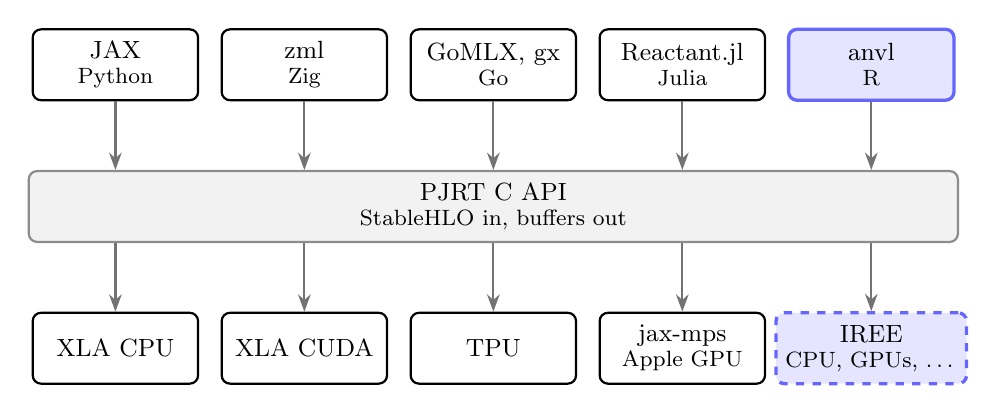
\begin{tikzpicture}[
  every node/.style={font=\small},
  box/.style={
    draw, rounded corners=3pt, thick,
    minimum width=2.1cm, minimum height=0.9cm, align=center
  },
  ours/.style={box, fill=blue!10, draw=blue!60, very thick},
  core/.style={box, fill=black!5, draw=black!45, minimum width=11.8cm},
  iree/.style={box, fill=blue!10, draw=blue!60, very thick, dashed},
  arr/.style={-{Stealth[length=2.2mm, width=1.6mm]}, thick, draw=black!55}
]
  \node[box]  (jax)  at (0,    3.4) {JAX\\[-2pt]{\footnotesize Python}};
  \node[box]  (zml)  at (2.4,  3.4) {zml\\[-2pt]{\footnotesize Zig}};
  \node[box]  (go)   at (4.8,  3.4) {GoMLX, gx\\[-2pt]{\footnotesize Go}};
  \node[box]  (jl)   at (7.2,  3.4) {Reactant.jl\\[-2pt]{\footnotesize Julia}};
  \node[ours] (anvl) at (9.6,  3.4) {anvl\\[-2pt]{\footnotesize R}};

  \node[core] (pjrt) at (4.8, 1.6) {PJRT C API\\[-2pt]{\footnotesize StableHLO in, buffers out}};

  \node[box]  (xcpu) at (0,    -0.2) {XLA CPU};
  \node[box]  (xgpu) at (2.4,  -0.2) {XLA CUDA};
  \node[box]  (tpu)  at (4.8,  -0.2) {TPU};
  \node[box]  (mps)  at (7.2,  -0.2) {jax-mps\\[-2pt]{\footnotesize Apple GPU}};
  \node[iree] (iree) at (9.6,  -0.2) {IREE\\[-2pt]{\footnotesize CPU, GPUs, \dots}};

  \foreach \f in {jax, zml, go, jl, anvl} \draw[arr] (\f.south) -- (pjrt.north -| \f.south);
  \foreach \p in {xcpu, xgpu, tpu, mps, iree} \draw[arr] (pjrt.south -| \p.north) -- (\p.north);
\end{tikzpicture}
\end{document}
